\documentclass{aa}
%\documentclass[referee]{aa} 

\usepackage{natbib}
\usepackage{graphicx}
\usepackage{color}
\usepackage{txfonts}
\usepackage{hyperref}
\hypersetup{colorlinks, allcolors=blue}

\usepackage[T1]{fontenc}
\usepackage{verbatim}
\usepackage{textcomp}
\usepackage{textgreek}

%________________________________________________________________

\newcommand{\brgamma}{\ion{Br}{$\gamma$}~}
\newcommand{\sig}{$\sigma$~}
\newcommand{\m}{$^\mathrm{m}$~}
\newcommand{\um}{$\mu$m~}
\newcommand{\ume}{$\mu$m}
\newcommand{\msun}{M$_\odot$~}
\newcommand{\msune}{M$_\odot$}
\newcommand{\s}{$\sim$}
\newcommand{\h}[1]{$^{#1}$}
\newcommand{\spa}{stars arcsec$^{-2}$~}
\newcommand{\spae}{stars arcsec$^{-2}$}
\newcommand{\needcite}{\colorbox{black}{\textcolor{yellow}{\textbf{Citation?}}}}
\newcommand{\correct}{\colorbox{red}{\textcolor{white}{\textbf{Correct?}}}}
\newcommand{\rewrite}{\colorbox{blue}{\textcolor{white}{\textbf{Re-write}}}}


%________________________________________________________________


\begin{document} 

  \title{The future of IMF studies with the ELT and MICADO\thanks{This work uses the instrument simulation package for MICADO, SimCADO: \url{https://simcado.readthedocs.io/}}}
  \subtitle{I: The local Universe as a resolved IMF laboratory}
  \author{K. Leschinski\inst{1}
     \and
          J. Alves\inst{1}
     }

  \institute{University of Vienna, Department of Astrophysics,
          Vienna, Austria\\
          \email{kieran.leschinski@univie.ac.at}
     }

  \date{Received TBD; accepted TBD}

      % 

\abstract
% context heading (optional)
% {} leave it empty if necessary
{Young stellar cluster cores in the local Universe provide the most pristine information available on the stellar Initial Mass Function (IMF), but their stellar densities are too high to be resolved by present-day instrumentation. With a resolving power 100 times better than the Hubble Space Telescope, the MICADO near-infrared camera on the Extremely Large Telescope (ELT) will provide access for the first time to a significant number of dense young stellar clusters critical to direct studies on the universality and shape of the IMF.}
% aims heading (mandatory)
{In this work we aim to estimate the lowest stellar mass that MICADO will be able to detect given a stellar density and distance robustly, and how many young clusters will be accessible for IMF studies in the local Universe with the ELT.}
% methods heading (mandatory)
{We used SimCADO$^1$, the instrument simulator package for the MICADO camera, to generate observations of 56 dense stellar regions with densities similar to the cores of young stellar clusters. We placed the cluster fields at distances between 8\,kpc and 5\,Mpc from the Earth implying core densities from 10\h2 to 10\h5\,\spa and determined the lowest reliably observable mass for each stellar field via PSF fitting photometry.}
% results heading (mandatory)
{Our results show that stellar densities of \textless10\h3\,\spa will be easily resolvable by MICADO. The lowest reliably observable mass in the LMC will be around 0.1\,\msun for clusters with densities \textless10\h3\,\spa. MICADO will be able to access the stellar content of the cores of all dense young stellar clusters in the Magellanic clouds, allowing the peak and shape of the IMF to be studied in great detail outside the Milky Way. At a distance of 2\,Mpc all stars with M\,\textgreater\,2\,\msun will be resolved in fields of \textless10\h4\,\spa, allowing the high-mass end of the IMF to be studied in all galaxies out to, and including, NGC\,300.}
% conclusions heading (optional), leave it empty if necessary 
{We show that MICADO on the ELT will be able to probe the IMF of star clusters 10$\times$ denser than what JWST will be able to access, and over 100$\times$ denser than those imaged by Hubble. While the sensitivity of MICADO will not allow us to study the brown dwarf regime outside the Milky Way, it will enable access to all stellar members of over 1000 young clusters in the Milky Way and the Magellanic clouds. Furthermore, direct measurements of the Salpeter slope of the IMF will be possible in more than 1500 young clusters out to a distance of 5\,Mpc. MICADO on the ELT will be able to measure resolved IMFs for a large ensemble of young clusters under starkly different environments and test the universality of the IMF in the local Universe.}



% * ELT PSFs make life very difficult - many fake sources
% * MICADO can get well into the Brown dwarf regime (>0.01Msun) for all clusters within 8kpc of the Sun
% * It will just miss out on the BD knee in the LMC (>0.1Msun). But it will catch the true structure of the 0.5Msun knee.
% * Densities of ~1000 stars/arcsec2 are easily resolvable. 5000 stars/arcsec2 if we have good knowledge of the PSF.
% * This is equivalent to every star in the Arches cluster at a distance of the LMC. ONC would be fully resolvable (assuming no extinction) in Leo I Dwarf (220kpc)
% * in the LMC, meaning MICADO can basically resolve out all stars in every YMC listen in Portegeis-Zwart 2010


% Current observations of the cores of densely populated clusters are severely limited by confusion as the stellar densities in the densest regions of clusters are often above one star per telescope FWHM.

% We used the MICADO instrument data simulator to generate a suite of images that mimic possible future observations with the ELT+MICADO. The images are of simulated open clusters and OB associations covering a range of cluster masses (100 to 10\,000 M$\odot$), radii (0.3 to 300 pc) and distances (1 kpc to 1 Mpc). We extracted the sources using a basic PSF-subtraction technique and compared the resulting IMF curves to the input models to determine the recovery fractions for various sets of initial parameters.


% Problem
    % IMF is only well studied for nearby clusters, further away crowding gets involved. Assumed to be constant
    % IMF is needed by all   
    
% Opportunity
    % ELT will give us resolving power and depth
    % This will allow us determine the IMF shape throughout the MW and in nearby galaxies

% Question we want to answer
    % What will the limits be for such IMF studies?
    % Down to what mass stars will we be able to observe?
    % How crowded can a region be for us to still observe 90% of the stars above the detection limit?
    % What effects do we need to be aware of when doing such studies?
    
% Experiment
    % Objects of interest were clusters of young stars: open clusters, young massive clusters, OB associations. 
    % Why, because they are young, i.e. a full IMF and little gas hopefully
    % OB associations because they are still young but easier to resolve

    % Simulate images of different stellar clusters that follow an IMF
    % Extract stars from the images and reconstruct the IMF

% Parameter Space    
    % Current limits are determined either by spatial resolution (HST) or Sky Background (AO observations at VLT)
    % Spatial resolution is currently at the diffraction limit of HST, at 0.1"
    % Depth and distance limit of 8m telescopes by atmospheric BG. For NACO and HAWK-I its around 24\m

    % What are typical densities of Young populations
        % Include graph where OC/OBA are plotted.
    % Depends on size, mass of cluster and distance from Earth
    % HST could comfortably resolve ~10 stars/arcsec (3 FWHM) and theoretically go up to ~100 stars/arcsec
    % NACO could resolve ~100 stars/arcsec comfortably, albeit over a small FoV
    % MICADO can do 10E3 stars/arcsec comfortably (3 FWHM) and push to 10E4

    % However as stars become too faint to be observed, they contribute to the background noise, but are no longer detectable. Hence effective stellar density decreases
        % Hence we scaled to 1E6 stars/arcsec

        % stellar densities
        % - 100 stars/arcsec2 --> 1E6 stars/arcsec2

    % Distance wise we're limited by the background. HST can go to J~28.5 (in a 10 hour observation). NACO/HAWK-I can get down to J~24 in a (1 hour observation). The interesting part of the IMF is around the 0.2-0.5 Msun region. So abs mags of J/K = 11.5/10.5 up to J/K = 7/6. Ground based telescopes are limited to distance moduli of 13 for the BD knee and 17 for the LM knee. This puts us at like 5kpc or 30kpc respectively with ground based scopes. HST can go to DMs of 17 (30kpc) and 21 (200kpc) for the BD and LM knees

    % We want to start at the ground based limits and push the limits. A list of nearby objects where we could investigate the IMF outside of our neighbourhood and the similar conditions that we find here. Realistically they are the closest galaxies and the galactic centre 

        % Distances
        % - 8kpc, 50kpc, 200kpc, 800kpc, 2Mpc, 5Mpc

% Instrument setup
    % Standard MICADO setup
    % K band because Strehl ratio is the best and we have absolute magnitudes for MS stars
    % Exposure time is set to 1 hour, just because
    % To save on computation time we only simulated a 2"x2" window near the centre of the FoV
        % This also meant that we didn't need to worry about the PSF varying over the field
    % Field of View make a 1/1E5 ratio: at 5Mpc, we're looking at a side length of 50pc. At 50kpc, we're looking at 0.5pc
        
    % Field of View : 2" x 2"
    % PSF : MAORY SCAO
    % Exposure time : 1 hour
    % Filter : Ks

% Cluster setup
    % n stars were sampled from an IMF for each density 
    % the distance modulus added to the absolute magnitudes of each star
    % Positions were assigned at random in the 2"x2" square
        % While this may not be a completely accurate representation of 

% Reduction steps
        

% Results
    % ELT PSFs make life very difficult - many fake sources
    % MICADO can get well into the Brown dwarf regime (>0.01Msun) for all clusters within 8kpc of the Sun
    % It will just miss out on the BD knee in the LMC (>0.1Msun). But it will catch the true structure of the 0.5Msun knee. 
    % Densities of ~1000 stars/arcsec2 are easily resolvable. 5000 stars/arcsec2 if we have good knowledge of the PSF. 
    % This is equivalent to every star in the Arches cluster at a distance of the LMC. ONC would be fully resolvable (assuming no extinction) in Leo I Dwarf (220kpc)
     % in the LMC, meaning MICADO can basically resolve out all stars in every YMC listen in Portegeis-Zwart 2010

% Discussion



% Cluster Age : 50 Myr (** should re-run for 5 Myr)

% IMF Variations :
% Cluster Mass : 1000

% For each section (M<0.08, 0.08<M<0.5, M>0.5), use standard alphas (0.3, 1.3, 2.3) and do +/- (0.1, 0.5)







% Background
% - What is the IMF and why are we interested in it?

% - What can MICADO, the ELT and SimCADO bring to this field?
  % IMF studies are currently limited by Seeing for ground based observations, or the diffraction limit of a 2.4m mirror for space based studies. This restricts studies to stellar densities of tens of stars per square arcsecond. In real terms, this means dense stellar environments like the cores of very young open clusters can only be investigated if they are very nearby (@give example). OB associations allow stellar populations at lerger distances to be studied, however these are also 
  

% - Why are we using Open clusters and OB associations? YMCs?
  % Mainly because they provide us uncontaminated environments to study the IMF
  % Open clusters are the birth places of stars, where almost all stars are still present. I.e. no Supernova. Gas only lasts for several ~Myr because of the OB stars. Once the gas is gone the clusters start to disperse. However the high mass stars (>20 Msun) live for around 100 Myr, so even though the stars disperse, we can still get a good handle on the full IMF by looking at the population of OB associations. The ultra high mass end of the IMF will not be recoverable, but that does not matter as the interesting stuff is what is happening around the 0.5Msun knee and into the BD regime.
  % Obviously the younger the better as then we have as many MS stars as possible. Though too young and we run into two issues - not all stars have formed and gas gets in the way of accurate mass/age determinations.
  % YMC are the best candidates because they provide us with a young environment where the high mass regions of the IMF are properly sampled, but also where enough of the low mass stars are present to get a proper handle on the actual shape of the LM/BD mass functions
  

% - What questions do we aim to answer in this study?

%    - At distance X and for stellar density Y, down to which mass (Z) can I get an IMF?
    
%    - If variations exist in the IMF, what level could MICADO detect at which distance?

% - What is new about this work
%  There have been many studies into the stellar populations 


  \keywords{}

\maketitle

%________________________________________________________________

%@arxiver{5_clusters.pdf,old_trusted_mass.pdf,resolved_stellar_densities.pdf}

\section{Introduction}
\label{sec:introduction}

\begin{table*}

    \centering
    \caption{A compilation of mass limits for a selection of studies of the IMF outside the Milky Way with the Hubble space telescope. It should be noted that for the study by \citet{gallart1999} the estimated global star formation history was consistent with a Salpeter slope, rather than a Salpeter slope being extracted from the photometric data.}
    \label{tbl:imf_lit_review}

    \begin{tabular}{ l l r r r r r }

        \hline
        \hline
        Galaxy   &  Target      &  Distance &  Mass range       & IMF Slope(s) & Break Mass          & Reference         \\
                &               & kpc       & \msun             &              & \msun               &                   \\
        \hline                  
        LMC      &  R136        & 50        & 2.8-15            & 2.22         &                     & Hunter 1995       \\
        LMC      &  NGC 1818    & 50        & 0.85-9            & 2.23         &                     & Hunter 1997       \\
        LMC      &  R136        & 50        & 1.35-6.5          & 2.28, 1.27   & 2.1                 & Sirianni 2000     \\
        LMC      &  LH 95       & 50        & 0.43-20           & 2.05, 1.05   & 1.1                 & Da Rio 2009       \\
        \hline                                                  
        SMC      &  NGC 330     & 62        & 1-7               & 2.3          &                     & Sirianni 2002     \\
        SMC      &  NGC 602     & 62        & 1-45              & 2.2          &                     & Schmalzl 2008     \\
        SMC      &              & 62        & 0.37–0.93         & 1.9          &                     & Kalirai 2013      \\
        \hline                                                  
        Hercules &              & 135       & 0.52-0.78         & 1.2          &                     & Geha 2013         \\
        Leo IV   &              & 156       & 0.54-0.77         & 1.3          &                     & Geha 2013         \\
        Leo I*   &              & 250       & 0.6-30            & 2.3          &                     & Gallart 1999      \\  
        \hline
        \end{tabular}

\end{table*}


The stellar Initial Mass Function (IMF), or the spectrum of stellar masses at birth,  has implications in almost all fields of astrophysics.  
On the local scale, the IMF determines the fate of a star formation region and determines the environment that emergent planet-forming circumstellar disks will be exposed too\needcite. 
On the large scale, the IMF is irrevocably connected to the composition of the stellar populations in a galaxy and has a massive impact on the mass and energy cycle of a galaxy. 
For example, the larger the amount of mass locked up in low mass stars, the smaller the reservoir of gas available for the next generation of stars and and consequently the smaller the potential for the enrichment of the interstellar medium (ISM)\needcite. 
Finally, cosmological simulations of galaxy formation and galaxy clusters inevitably rely on a universal the IMF to determine stellar yields and the strength of feedback mechanisms governing the transport of energy and material\needcite. 
In short, the IMF is a fundamental parameter in astronomy. 

% In his original work, \citet{salpeter1955} used a single power law distribution with a slope of 2.35 to describe the IMF for masses greater than \s1\,\msun. This was later modified to a series of broken power laws to include the stars below the hydrogen burning limit by \citet{kroupa2001}. In contrast, \citet{chabrier2003} proposed a log-normal distribution with a power law modification for the high and low mass regions. As the two descriptions are very similar in the most populated region between 0.1\msun and 10\msune, it has proved  difficult to decide which model more aptly describes the IMF.

In his original work, \citet{salpeter1955} used a single power-law distribution with a slope of 2.35 to describe the IMF for masses between \s1\ and \s10\,\msun . This description was later modified to a series of broken power laws to include the stars below the hydrogen-burning limit by \citet{kroupa2001}. \citet{chabrier2005} proposed a log-normal distribution with a power-law modification for the high and low mass regions. Although not an important goal per se, as both descriptions are empirical and not the prediction of a theory, it has proved difficult from observations to decide which of these two descriptions more aptly describes the IMF.

Most observational studies suggest that the shape of the IMF is constant \citep{Kroupa2002,Bastian2010}. 
Definitive deviations from the accepted IMF form are elusive, and when found, often controversial\needcite. 
Still, there is one major aspect that hinders general acceptance of a universally constant IMF: a lack of IMF estimate derived directly from star counts for environments substantially different from the solar neighbourhood. 
Table \ref{tbl:imf_lit_review} shows that even in the closest star forming galaxies like the Magellanic clouds, only the Hubble space telescope (HST) has the sensitivity to reach below one solar mass (see references in Table \ref{tbl:imf_lit_review}). 
Long exposures with HST have observed stars just below the first break in the Kroupa power law at 0.5\,\msun \citep{dario2009,kalirai2013,geha2013}, but not far enough into the lower mass regions to put reliable constraints on the shape of the IMF in these extragalactic environments. 
Adding to observers' woes is the lack of spatial resolution. At the distance of the LMC, star forming regions can contain anywhere from 10\h2 to 10\h5\,\spa. 
Figure~1 of \citet{sirianni2000} shows a perfect example of why current studies struggle to reliably determine the IMF for dense stellar populations outside the Milky Way. The depicted cluster core (R136) is completely dominated by the flux of a few of the brightest stars.
Thus studies of the IMF are limited to the outer regions of these clusters where stellar densities are low enough for individual low mass stars to be resolved. 
The age of a cluster and the resulting level of mass segregation can also skew the results when considering the IMF in massive clusters \citep{lim2013}\needcite. 
However without being able to study the core of such clusters in- and outside the Milky Way, it is difficult to determine to what extent this plays a role. Thus in order to systematically study the lower mass, and arguably most interesting, part of the IMF telescopes with higher spatial resolution and better sensitivity than the current generation of ground and space based telescope will be needed.

In the middle of the next decade, the era of the extremely large telescopes will begin. 
ESO's Extremely Large Telescope (ELT) \citep{eelt} with the help of advanced adaptive optics \citep{maory} will have the power to resolve spatial scales at the diffraction limit of a 40m-class mirror. This will provide an improvement of a factor of \s15$\times$ over HST and a factor of \s6$\times$ over the future JWST telescope. 
With a collecting area of 978\,m\h2 the ELT will have at least the same sensitivity as the HST in sparse field and will be able to observe much deeper than HST in crowded fields. 
The MICADO instrument \citep{micado, micado2016} will be the ELT's first-light near-infrared (NIR) wide-field imager and long slit spectrograph. 
With a diffraction limit of 7\,mas at 1.2\um and an AO corrected field of view of almost a square arcminute, MICADO will be perfectly suited to address exactly this niche. 

The main focus of this paper is to determine to what extent MICADO will improve our ability to study the IMF and other properties of dense stellar populations is the main focus of this paper. 
In this paper we have attempted to addressed the following two questions: What is the lowest mass star that MICADO will be able to observe for a given density and distance?
What instrumental effects will play a critical role when undertaking such studies with MICADO and the ELT?
%How crowded can a region be for MICADO to still be able to detect 90\% of the stars above the detection limit? 
In our quest for answers we used SimCADO, the instrument data simulator for MICADO \citep{leschinski2016}, to simulate a wide range of densely populated stellar fields at various distances. 
The current version of SimCADO takes into account all the major and most of the minor spatial and spectral effects along the line of sight between the source and the detector. 
We used the software to generate realistic images of our model stellar fields and  conducted several iterations of PSF photometry and star subtraction to extract as many stars as possible from the simulated observations. 
The extracted stars were compared with the input catalogue to determine the completeness of the extraction and to define a ``limiting reliably observable mass'' for the different stellar field densities and distances.

This paper is organised in the following way: Section \ref{sec:observations} describes the stellar fields used in our simulations, how the simulations were run, and also describe the algorithm for detecting and subtracting stars in the simulated images. 
In Section \ref{sec:results} we describe the results of the simulations and discuss their validity in the context of possible future observations of real young stellar clusters. 
Section \ref{sec:conclusion} summarises our results.

\section{Data sets}
\label{sec:observations}


\begin{figure*}

    \centering
    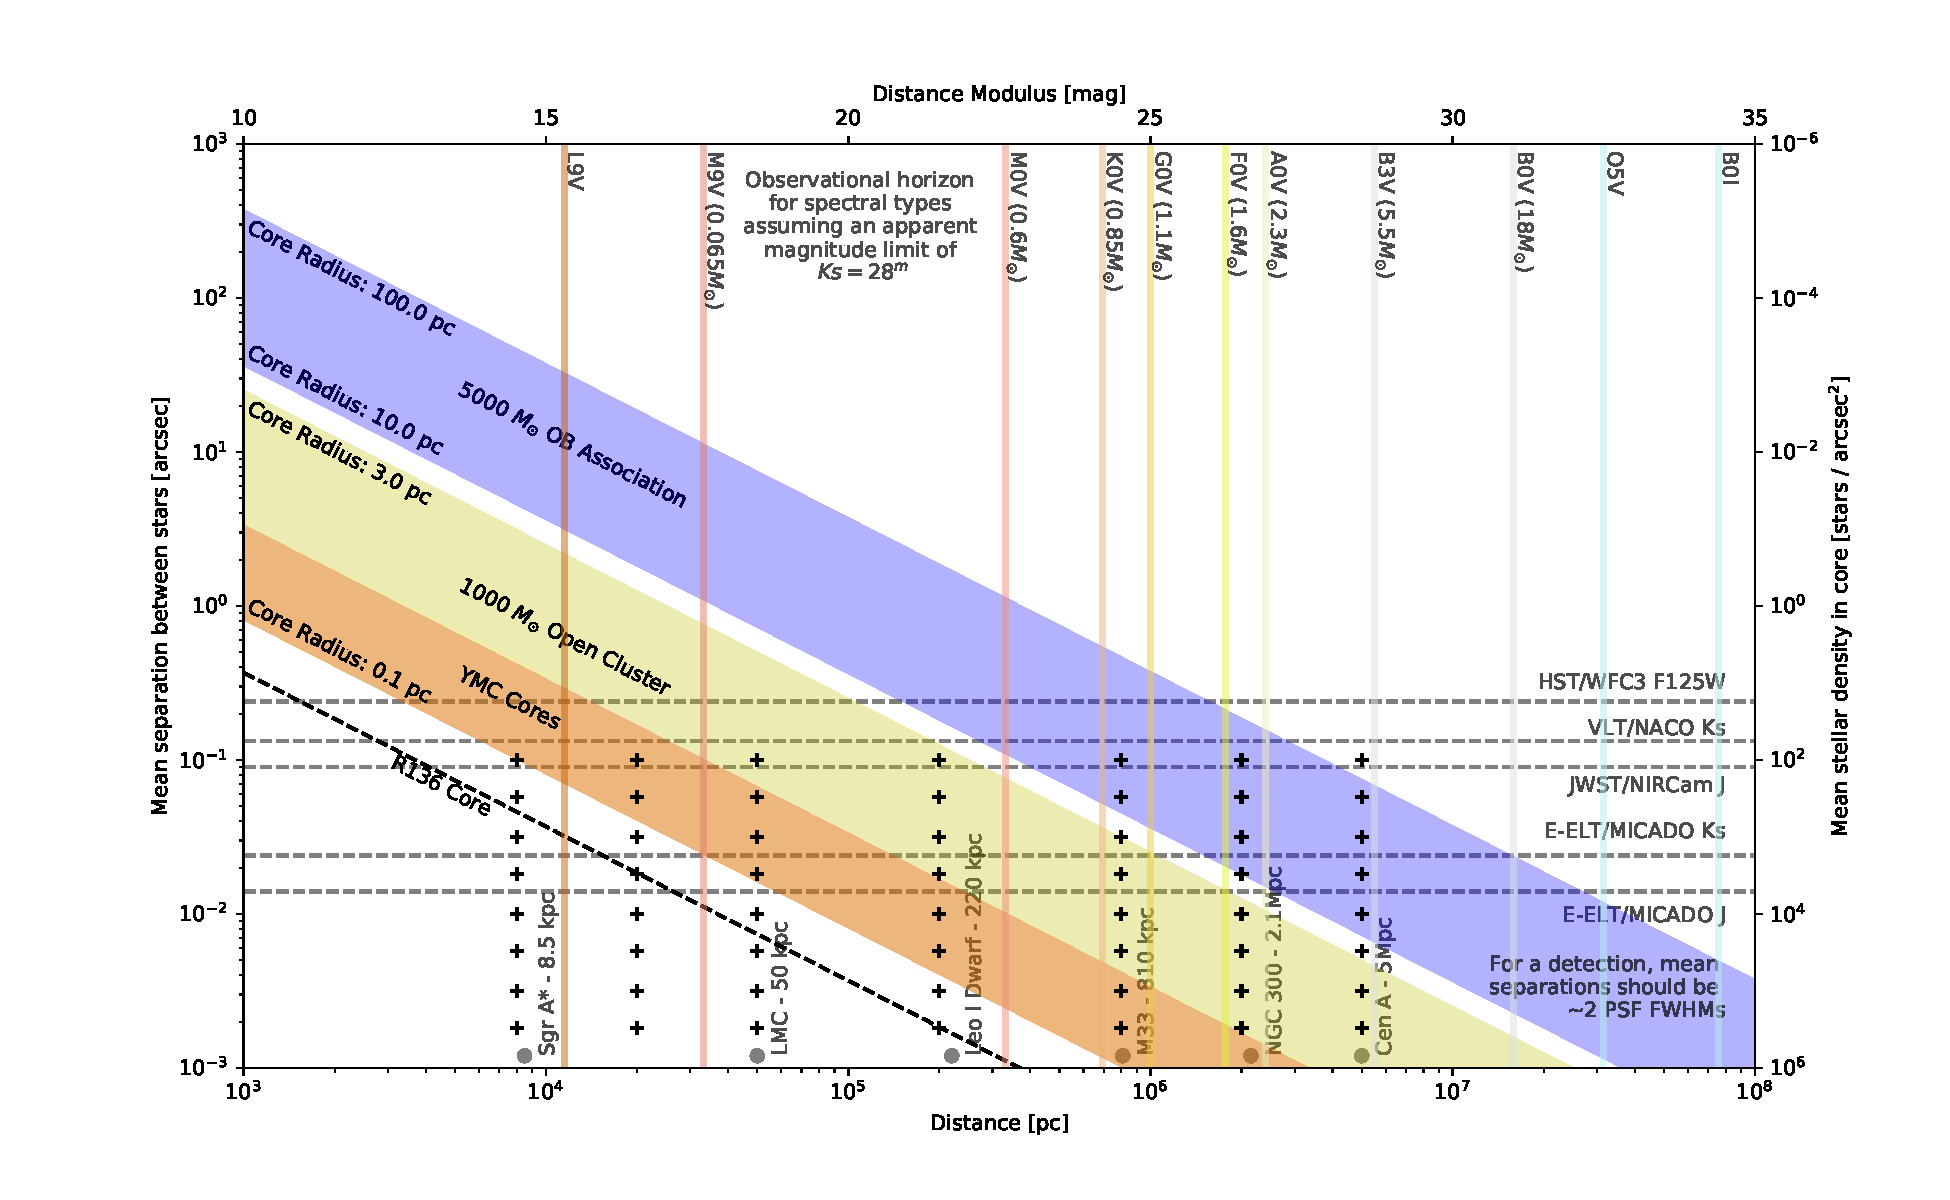
\includegraphics[width=\textwidth]{images/resolved_stellar_densities}

    \caption{The on-sky stellar density parameter space covered by the dense stellar fields in this study (crosses). 
    The diagonal bands show the range of core stellar densities for the three major categories of young stellar populations: young massive clusters (orange), open clusters (green), and OB associations (blue). 
    The vertical lines represent the furthest distance at which a certain type of main sequence star will still be above the detection limit of MICADO, i.e. Ks=28\m.
    The dashed horizontal lines show the theoretical confusion limit for MICADO/ELT, JWST, HST and an instrument similar to NACO/VLT. The confusion limit assumes an average minimum distance of 2$\times$ the PSF FWHM between stars.
    }
    
    \label{fig:resolved_stellar_densities}
    
\end{figure*}

\rewrite INCLUDE GRID OF POSTAGE STAMPS FOR CLUSTERS

The most reliable way to determine the IMF is to look at a population of stars which is still young enough for all the original members to still be around, yet old enough that the main phase of star formation activity has ceased\needcite. 
If a population is too young, it will not have finished forming all its stars and dust extinction will be a major source of uncertainty and incompleteness. Too old and the most massive members will already have exploded as supernovae. 
Dynamical effects will also have led to evaporation of stars from the cluster. 
Unfortunately such ideal conditions are rarely observed. 
Star formation happens on time scales of 10\h6 years. 
The most massive stars burn their hydrogen reserves within the first several ten million years and move off the main sequence\needcite. 
Given that the dispersion time for stellar clusters is on the order of hundreds of millions of years, at any point in time relatively few of the observable new clusters will be found in the ideal age range (between 5 and 20\,Myr) for studying the IMF\needcite. 
The majority of IMF studies focus on the clusters which come closest to meeting these conditions - namely the cores of open clusters (OC) and young massive clusters (YMC)\needcite. 
It should be mentioned that OB associations also provide a laboratory for studying the IMF. 
However as these are older and in many cases more spread out, the chances of contamination from background sources and missing ejected stars is higher\needcite\correct. 
Furthermore, the high mass end of the IMF cannot be reliably observed as the highest mass stars have already left the main sequence, and some have ended as supernova\correct.


\subsection{Parameter Space}

HST has a diffraction limit of \s0.1'' at 1.2\,\um and can reach magnitudes as faint as J=28.6\m \citep{hst_wfc3} in a 10 hour observation. Using AO assisted ground based instruments similar to NACO at the VLT, diffraction limited observations can be achieved over small (\s1') fields of view. 
The diffraction limit of the VLT telescopes (\s0.03'' at 1.2\,\um) is 3$\times$ smaller than HST, however due to the atmospheric background the sensitivity limits of VLT instruments are many magnitudes brighter than for HST. 
As boundary conditions for our suite of stellar fields we took the resolution limit of HST, as cluster cores with densities lower than this are already accessible to the HST. 
Assuming an average of one star per FWHM of the PSF, our lower density limit was set to 100\,\spa. 
For the upper density limit we first took the theoretical diffraction limit of the ELT: 7\,mas at 1.2\,\ume, or 2$\times$10\h4\,\spae. However as faint stars drop below the telescope's detection limit the effective density of detectable stars decreases with increasing distance. 
As we wanted crowding limited observations at large distances (\textgreater1\,Mpc), we increased the true stellar density by a factor of 15$\times$ so that the M\,\textgreater\,1\,\msun stars alone would meet the crowding criterion of 1 star per FWHM. 
Thus we set the upper limit for the true cluster stellar density to 3$\times$10\h5\,\spa.

Current telescopes are capable of detecting almost all main sequence stars above the hydrogen burning limit (\s0.08\,\msune) within a few kiloparsecs of the Sun\needcite. 
Detecting all main sequence stars in clusters further afield, e.g. in the galactic centre and beyond, is where MICADO's increased sensitivity and resolution will bring the greatest breakthroughs. 
Indeed the question of whether the IMF is truly universal\correct dictates that we study the IMF outside the Milky Way. 
Therefore we placed our model proxy-clusters at distances corresponding to some of the more well known celestial landmarks: The Galactic Centre (\s8\,kpc), the LMC (\s50\,kpc), Leo I dwarf galaxy (\s200\,kpc), M33 (\s800\,kpc)\footnote{The author recognises that the location of the ELT in the southern hemisphere is unfavourable for effectively observing M33. We provide this data point because M33 will, with luck, be visible to the Thirty Meter Telescope.}, NGC 300 (\s2\,Mpc), and Cen A (\s5\,Mpc). 
Figure \ref{fig:resolved_stellar_densities} shows the parameter space covered by open clusters of average mass (\s1000\,\msun) with radii between 0.1\,pc and 3\,pc and OB Associations of average mass (\s5000\,\msun) with radii between 10\,pc and 100\,pc as distance from Earth increases. 
The lower bounds of the open cluster parameter space also covers the cores of YMCs. Average cluster properties were derived for the OB Associations from \citet{melnik1995}, for the open clusters from \citet{piskunov2007}, and for the YMCs from \citet{portegies2010}.



\subsection{Artificial stellar fields}

In this study we generated densely populated stellar fields, that could function as proxies for the dense regions at the cores of young stellar clusters. 
The parameter space covered by these cluster proxies are shown with the crosses in Figure \ref{fig:resolved_stellar_densities}. 
The size of each stellar field was set at 2''$\times$2'' (see section \ref{sec:telescope}). 
The stellar fields were populated by continually drawing stars from an IMF until the required stellar density was reached. 
The mass of each star was drawn at random from an IMF distribution with minimum and maximum masses of 0.01\,\msun and 300\,\msun. 
The IMF followed a standard \citet{kroupa2001} broken power law distribution with breaks at 0.08\,\msun and 0.5\,\msun and standard slope exponents\footnote{By ``standard'' we mean: $\alpha=0.3$ for $\mathrm{M} < 0.08 \mathrm{M}_\odot$, $\alpha=1.3$ for $0.08\mathrm{M}_\odot < \mathrm{M} < 0.5 \mathrm{M}_\odot$, and $\alpha=2.3$ for $\mathrm{M} > 0.5 \mathrm{M}_\odot$ as defined in Kroupa (2001)}. 
The absolute J and Ks magnitudes for each star were calculated by interpolating Table 5 in \citet{pecaut2013}\footnote{Masses are not given in Table 5, but rather in the online suppliment at \url{http://www.pas.rochester.edu/~emamajek/EEM_dwarf_UBVIJHK_colors_Teff.txt}} for the given mass. 
The requisite distance modulus for the stellar fields was added to give each star an apparent magnitude. 
It should be noted that we did not include extinction in the distance modulus as this varies with the line of sight. 
The stars were assigned random coordinates within the 2''$\times$2'' bounding box. 
Although true clusters follow a radial luminosity profile, and hence density profile, for this study we were primarily interested in the densest regions, i.e. the worst case scenario. 
Hence distribution of stars in our stellar fields followed a uniform random distribution. 
In real observations the decline in density with radial distance will most likely result in a better characterisation of the IMF over our pessimistic approach.

%\section{Simulations and data analysis}

\subsection{Observations}
\label{sec:telescope}

To ``observe'' our stellar fields we used the standard imaging mode of SimCADO \citep{leschinski2016} which mimics observations with the wide-field mode of MICADO at the ELT. 
The core regions of open clusters and YMC have radii on the order of \s1\,pc \citep{portegies2010}. 
At a distance of 200\,kpc ($\sim$Leo 1 Dwarf), this translates to an angular diameter of \s2''. Thus we thought it safe to assume that the stellar density within the inner 2''$\times$2'' region should remain relatively constant.
For the sake of computational effort we decided to restrict to observations to this 2''$\times$2'' window in the centre of the detector.

At the very least dual-band photometry is required to determine the mass of a star. Therefore detections in at least the J and K$_S$ filters are necessary. 
We deemed a detection in the K$_S$ filter to be critical for any study of the IMF and therefore restricted our observations to this filter. 
The reason for this is as follows: The sky background in the K$_S$ filter is the highest of all NIR filters and the NIR stellar flux is for all main sequence stars (and many brown dwarfs) weakest in the K$_S$ filter. 
If a source is undetectable in the K$_S$ filter it will not be possible to determine its mass accurately. Given the AO-nature of the observations and the expected low Strehl ratio at 1.2\um \citep{clenet2016}, it could be argued that detections in the J filter will be more difficult. 
Ultimately the fluxes of the stars and the sky are set by nature, whereas the Strehl ratio is a question of engineering and optical design. 
The stars cannot be made brighter, whereas optical quality can be improved. 
Hence we deemed a detection in the K$_S$ filter to be the critical point for determining the mass of cluster members.
%This assumption comes with its own set of problems which will be discussed in a later paper.

Exposure times were kept to 1 hour for no other reason than observing time at the ELT will be in very high demand once it comes on line and observations in two or more filters are needed to accurately determine the mass of stars.


\subsection{Source extraction and matching}
Figures \ref{fig:results_lmc_1E3} and \ref{fig:results_lmc_1E4} in the Appendix show a graphical representation of the process described in this section. 
They show two examples of ``observed'' stellar fields placed at a distance of 50\,kpc and containing 10$^3$ and 10$^4$ \spa respectively. 
The stark features of the SCAO PSF\footnote{The PSF user here was from a simulation of the SCAO mode from MAORY. It was only released internally within the MAORY consortium. By default the SimCADO package comes with a SCAO PSF generated by the MICADO consortium, which is in the public domain.} are clearly visible in the images. 
The diffraction core of the PSF is however still well modelled by a Gaussian distribution.
To find and measure the stars in the images we used the following method:

\begin{enumerate}
    \item Find the brightest star in the image with \verb+DAOStarFinder+ from \verb+photutils+ \citep{photutils}
    \item Find the centre of the star in a 5$\times$5 pixel window around the coordinates given by \verb+DAOStarFinder+
    \item Fit a 2D Gaussian profile to the core of the star
    \item Scale an image of a reference star to match the amplitude, baseline and offset of the found star
    \item Subtract the scaled reference star from the image
    \item Repeat until \verb+DAOStarFinder+ no longer finds any sources above 5\,\sig
\end{enumerate}

In practice we found that we could subtract \s100 stars at once and thus greatly increase the speed of the process. 
The amplitudes and baselines were converted to magnitudes based on the reference star. 
Our reference star was a solitary ``field'' star with a magnitude of K$_S$=15, observed for the minimum {MICADO} exposure time of 2.6\,s so as to maximise the signal-to-noise ratio while not saturating the detector. 
We calculated the mass of each star based on the observed fluxes in the K$_S$ filter. 
This step is only permissible because of the simplified context of this study. 
We were free to equate the luminosity function with an equivalent mass function because all our stellar fields have the intrinsic property that they only contain main sequence stars and the luminosity and mass functions enjoy a one-to-one relationship for this conversion in the K$_S$ filter, mathematically speaking. 
Furthermore, our primary goal is to determine what the lowest reliably observable mass is, based on how well MICADO will perform in crowded fields - not to directly measure the mass of the original stars. 
We are confident that this step does not significantly detract from achieving the goal of this study\correct.

% We fitted the gaussian by flattening the star and the control star arrays, then doing linear regression to find the slope and intercept. We did this using scipy thielslope

Finally we cross-matched the coordinates of the extracted sources with the original table of coordinates to determine what fraction of stars were correctly detected with our algorithm. 
Due to noise and confusion from stars closer that a few FWHMs the centroid coordinates of the extracted star was not always exactly equal to the original coordinates. 
The cross-matching algorithm was instructed to search for the closest star within a 25\,mas radius. 
If a fainter or brighter star happened to be closer, then the algorithm chose that star from the catalogue as the match. 
We determined whether the extracted masses for stars in a certain mass bin were ``reliable'' by binning the extracted stars according to mass. 
We then took the mean and standard deviation of all stars within a mass bin. 
As long as the mean extracted mass to true mass ratio was in the range 1.0$\pm$0.1 and the standard deviation was less than 0.1, the mass bin was classed as reliable. 
By this definition the lowest reliably detectable mass for a stellar field was given by the lower edge of the lowest mass bin which satisfied these criteria.






































\section{Results and Discussion}
\label{sec:results}

\subsection{The lowest reliably observable masses for given stellar densities
and distances.}

\begin{figure*}

    \centering
    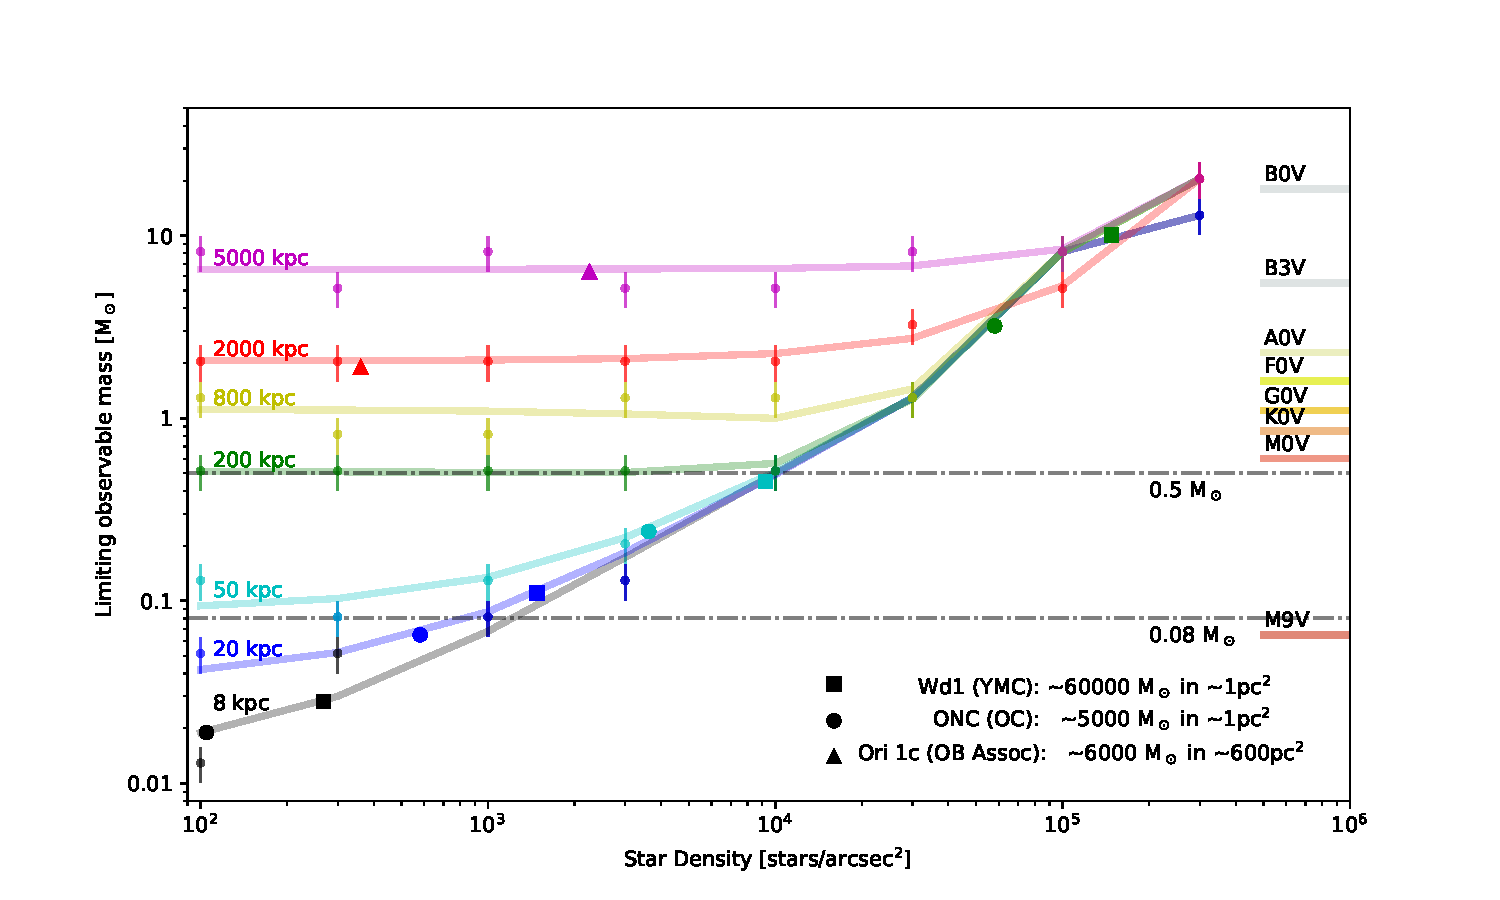
\includegraphics[width=\textwidth]{images/old_trusted_mass.pdf}

    \caption{This graph is the answer to the first question we posed: what is the lowest observable mass for given stellar densities and distances? 
    The errors in the observable mass are 0.2 dex and correspond to the size of the mass bins used. 
    Two trends are visible in the best fit lines for each distance: the flat regime shows that the limiting mass is based on the sensitivity limit of MICADO, while the exponential regime shows where crowding becomes the limiting factor. 
    The cavity to the lower right shows the parameter space in which stars of a given mass will not be observable.
    Here the stellar density includes all the stars in a given area down to 0.01\,\msun, not just the stars above the sensitivity limit. 
    Hence for the cases where observations are sensitivity limited, the effective observable star density is, in the cases with greater distance, much lower. 
    In these cases the stars below the sensitivity limit only contribute to a higher background flux.}
    
    \label{fig:trusted_mass}
    
\end{figure*}

\begin{figure*}

    \centering
    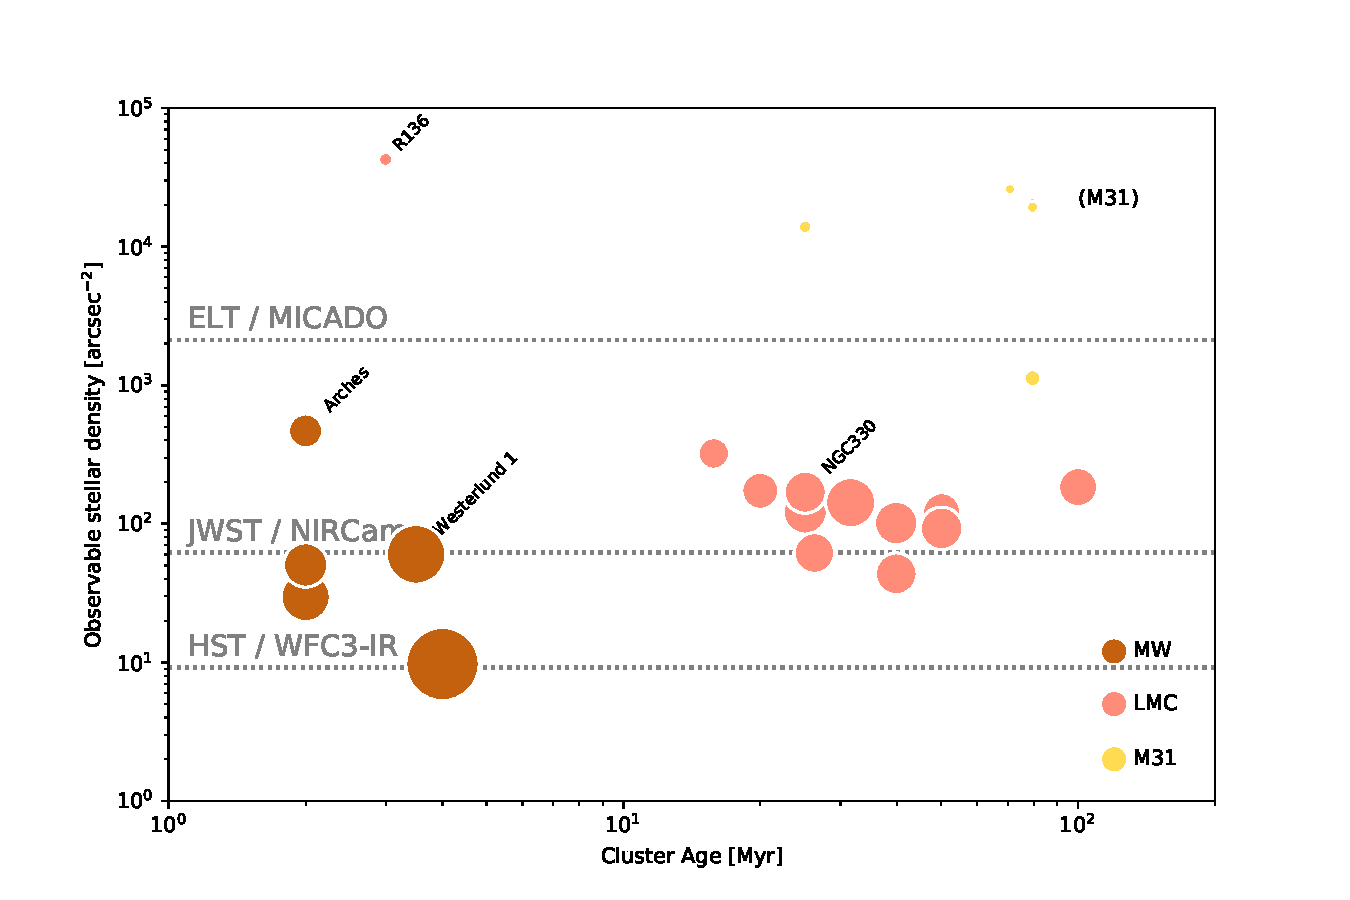
\includegraphics[width=\textwidth]{images/star_density_vs_age.pdf}

    % Add reference to that this is all-sky sample of YMCs
    % Note that all clusters apart from M31 will be accessible to MICADO

    \caption{\rewrite IS THIS GRAPH NECESSARY? 
    The stellar densities in the cores of the clusters listed in Table \ref{tbl:pz10_selection} assuming a sensitivity limit of K$_S$=28\m. 
    The size of the circles is proportional (including an offset) to the relative on-sky size of the cluster cores. 
    The colours reflect the lowest possible reliably observable mass, as shown in Figure \ref{fig:trusted_mass} and listed in Table \ref{tbl:pz10_selection}. 
    Brown: M\textgreater0.01\msun; Pink: M\textgreater0.1\msun; Yellow: M\textgreater0.9\msun. 
    The densities shown here take into account the sensitivity limit and therefore are only for the potentially observable stars, i.e. any low luminosity stars with K$_S$\textgreater28\m are omitted from the density calculation. 
    This is equivalent to all stars in the Milky Way, M-class stars and brighter in     the LMC, and G-class stars and brighter in M31. 
    Only clusters from \citet{portegies2010} which have a defined core radius, r$_c$, are shown.
    The dashed lines in this figure represent the (estimated) limit to the resolving capability of the HST, JWST and ELT. 
    We define the limiting density as the mean distance between stars being equal to 2$\times$ the H-band PSF FWHM.
    Given the predicted PSF shapes for the latter two telescopes, these lines may prove to be somewhat optimistic. 
    Nevertheless the graphic illustrates the point that cores of the majority of young clusters outside the Milky Way are far too dense for either HST or JWST observations.
    Thus it will require the ELT (or similar) to study the most heavily populated regions of these clusters.}
    
    \label{fig:star_density_vs_age}
    
\end{figure*}


The first of the questions we asked with this study -- ``What is the lowest mass star that MICADO will be able to observe reliably for a given density and distance?'' -- can be answered by Figure \ref{fig:trusted_mass}. 
For each of the distances and densities we have plotted the lowest reliable mass bin. 
The scatter in the plot reflects the random nature of the simulations. 
The positions of the stars in each of the stellar field were randomised, the sampling of the mass function was random and detector and shot noise was applied to the image as part of SimCADO's read-out process. 
Thus no two stellar fields were the same. 
Each stellar field configuration was only run once. 
We therefore only have one data point for each density and distance. 
The bin size used for the reliability statistics was set to 0.2 dex, and is the uncertainty in the limiting observable mass.

From Figure \ref{fig:trusted_mass} we can immediately see the two limiting regimes of sensitivity and crowding. 
The flat parts of the curves in Figure \ref{fig:trusted_mass} show the densities for which MICADO will be sensitivity limited at each distance and the diagonal regions show when crowding becomes the limiting factor. 
For example observations of a cluster at a distance of 8\, kpc observations will always be crowding limited for densities above 100\,\spae.
At a distance of 200\,kpc observations will be limited by sensitivity up to a density of 10\h4\,\spa, thereafter crowding will be the dominant factor. 
At 5\, Mpc all observations will be sensitivity limited. 
As a reference we have included the approximate stellar densities for three well known young  clusters in Figure \ref{fig:trusted_mass} \textit{if they were located at the distance of the simulated clusters}. 
For example, if the YMC Westerlund 1 were to be located in the LMC, it would fall in to the crowding-limited regime for MICADO.
The lowest reliably observable mass in the densest region of the core would only be \s0.5\,\msun. 
This is equivalent to what HST is capable of observing in the outer rim territories of LMC clusters. For clusters in the LMC with stellar densities less than 10\h3\spa MICADO will be limited by sensitivity to masses above 0.1\,\msun. 
While this mass is only 0.3\,\msun lower than what current Hubble observations can achieve, it should be emphasised that this increase of ``only'' 0.3\,\msun will reveal the majority of M-type stars, which account for almost three quarters of all main sequence stars \citep{ledrew2001}. 
Given that the limit of current studies is around the 0.5\,\msun knee from \citet{kroupa2001}, opening up this range will allow future studies to pin down exactly what the shape of the IMF looks like in the dense cores of young LMC clusters.

As previously noted the exposure time for the simulated images was one hour. 
By observing for longer times, the lowest observable mass will decrease, however the change is disproportionate to the exposure time. 
\citet{leschinski2016} show that increasing the exposure time from 1 to 10 hours per cluster only increases the sensitivity limit by around 1.5\m and 1\m in the J and K$_S$ filters respectively. 
For the case of the LMC, this would decrease the lowest observable mass to around 0.06\msune, i.e. just below the hydrogen burning limit.

It should be noted that the majority of young clusters have cores less dense than that of Westerlund 1, and therefore the limiting observable mass will also be lower than the 0.5\,\msun mass quoted for a Westerlund 1-like YMC in the LMC. 
Given MICADO's resolving power it will therefore also be possible to determine to what extent apparent mass segregation has played a role in previous studies of the IMF in the LMC.\needcite 
More to the point MICADO will enable us to understand the apparent deviations from the Salpeter IMF as reported by \citet{dario2009}, \citet{geha2013} and \citet{kalirai2013}.

% At these distances MICADO **would** be able to 
% Mention that ideal case is not possible, but that the older population can be resolved between 100-and 200 kpc down to 0.5 Msun

At distances of 100\,kpc to 200\,kpc and with careful photometry and longer observations MICADO should be able to detect stars down to the sensitivity limit of 0.5\,\msun. 
This will only be possible though for clusters with stellar densities less than 10\h4 \spa. 
As a reference an ONC-like cluster at a distance of 200\,kpc will have a stellar density on the order of 10\h5 \spa. 
Such observations will be useful for determining the composition of OB associations and sparser (older) open clusters, if there were any present in the non-Magellanic satellites of the Milky Way. 
Nevertheless MICADO will still allow us observe the fabled 0.5\,\msun knee in the field population of the nearest low metallicity dwarf spheroidal galaxies.\rewrite IS THIS SECTION NEEDED AS THERE ARE NO YOUNG CLUSTERS IN THESE GALAXIES

Closer to home MICADO should be able detect 10\,M$_{Jup}$ objects in a ONC-like clusters at a distance of 8\,kpc (along low extinction lines of sight). 
An obvious candidate for studies of the IMF in extreme environments is the Arches cluster, given its proximity to the galactic centre.
The main hindrance to deep observations of the Arches cluster is, somewhat counter-intuitively, not the \textgreater2 magnitudes of variable Ks-band extinction along the line of site \citep{espinoza2009}, but rather the \textgreater350 stars in the cluster \citep{galacticnucleaus} brighter than the saturation limit for MICADO\footnote{A MICADO internal analysis shows that point sources with magnitudes K$_S$\textgreater14.8\,\m will saturate the MICADO detectors within the 2.6\,s minimum exposure time.}.
Indeed there are very few regions in the cores of Milky Way open clusters which do not contain stars brighter than the saturation limit, making deep MICADO observations of these regions difficult.


\subsection{The core densities of young star clusters}

The second of the questions we asked with this study was ``What instrumental effects will play a critical role when undertaking such studies with MICADO and the ELT?''. 
The instrumental effect which plays the largest role by far regarding the accuracy of the estimates given here is our knowledge of the PSF.
For this study we used a single SCAO PSF. 
We assumed that the PSF orientation stayed the same for the length of the observation.
Consequently we had a very good model of our reference star for the PSF subtraction. 
This will obviously not be the case for real observations as the pupil of the telescope will rotate with respect to the sky, causing an axial broadening of the PSF over the course of an observing run. 
This broadening should improve the results from our subtraction method as it will smooth out many of the sharp features of the instantaneous PSF that lead to false positive detections. 
Information on both the structure of the PSF and the extent of the wings will however be lost due to the rotational broadening. 
Thus the PSF subtraction algorithm will less accurately be able to estimate the background level when fitting the reference PSF to a star. 
As a consequence faint stars caught in the PSF wings of the brighter stars may not be detected as often as they would be if the PSF remained rotationally aligned with the sky. 
To extract the most stars possible given the shape of the ELT PSF we propose the following hybrid approach: Subtract the brightest stars from each individual exposure using an instantaneous PSF derived from the brightest stars in that exposure, then stack the residual images and extract the faintest stars using a rotationally broadened PSF.
Further investigation is required to determine whether this approach would indeed increase the detection rate for faint stars.\rewrite

Although it may seem obvious, it is worth mentioning that regardless of the PSF shape, it is clear from our simulations that resolving stellar densities of 10\h3\,\spa is well within the capabilities of MICADO. 
With an optimised PSF fitting and subtraction algorithm, extracting upwards of 5$\times$10\h3\,\spa should also be in the realms of possibility. 
5$\times$10\h3\,\spa is equivalent to approximately one star in an area equivalent to \s2.5 ELT H-band PSF FWHMs. 
This is similar to being able to resolve every star in the core of an ONC-like cluster in the LMC. 
For JWST and HST the equivalent stellar densities are only 160~\spa and 20~\spa respectively. 
Although MICADO may not have the sensitivity of a space-based telescope, the resolving power will give us full access to the core populations of dense stellar clusters in the major satellites of the Milky Way.


\subsection{Opportunities and targets for future observations with MICADO and the ELT}

These simulations are a nice theoretical exercise, however without an application to observations they are not all that useful.
Figure~\ref{fig:star_density_vs_age} shows the estimated stellar densities in the cores of the open clusters and YMCs compiled by \citet{portegies2010}. 
The density values, log$_{10}$($\rho$), only take into account the stars with apparent magnitudes above the sensitivity limit of MICADO and thus reflect the ``real'' observable density for the clusters (also listed in Table \ref{tbl:pz10_selection}). 
The limits set for HST, JWST and MICADO are the critical stellar density above which our extraction algorithm struggles to detect and remove more than 90\% of the stars in a field. 
We find that for the Galactic clusters, the resolution of JWST will be sufficient to resolve all stars in most cluster cores down to the sensitivity limit of the instrument.

For clusters in the galactic plane though JWST observations will struggle to disentangle the cluster stars from the field stars. 
To robustly determine cluster membership, observations of the proper motion of the cluster relative to the field will be required. 
\citet{stolte2008} show that the proper motion of the Arches cluster near the Galactic centre is \s5\,mas yr\h{-1}. 
This equates to around a sixth the size of a pixel in the JWST NIRCam instrument. 
MICADO, in contrast, will have a plate scale of 1.5\,mas in the high resolution mode, meaning that cluster membership could be determined by observations spaced only several months apart. Greater certainty regarding cluster membership will greatly increasing the accuracy of estimates of the cluster IMF based on star counts.

Further afield, resolving the cores of the massive young clusters in the Magellanic clouds will not be possible with JWST. MICADO however will enable access to these cluster cores, which in turn will open up to possibility to study the dynamical processes (e.g. evaporation, core collapse, etc.) involved in the evolution of extra-galactic clusters. 
Additionally observations of a series of LMC clusters with varying ages will give a much better picture of how the initial mass function evolves into the present day mass function, and how the dynamical evolution of the cluster influences the observations, and calculations of, a cluster's IMF.

\begin{figure*}

    \centering
    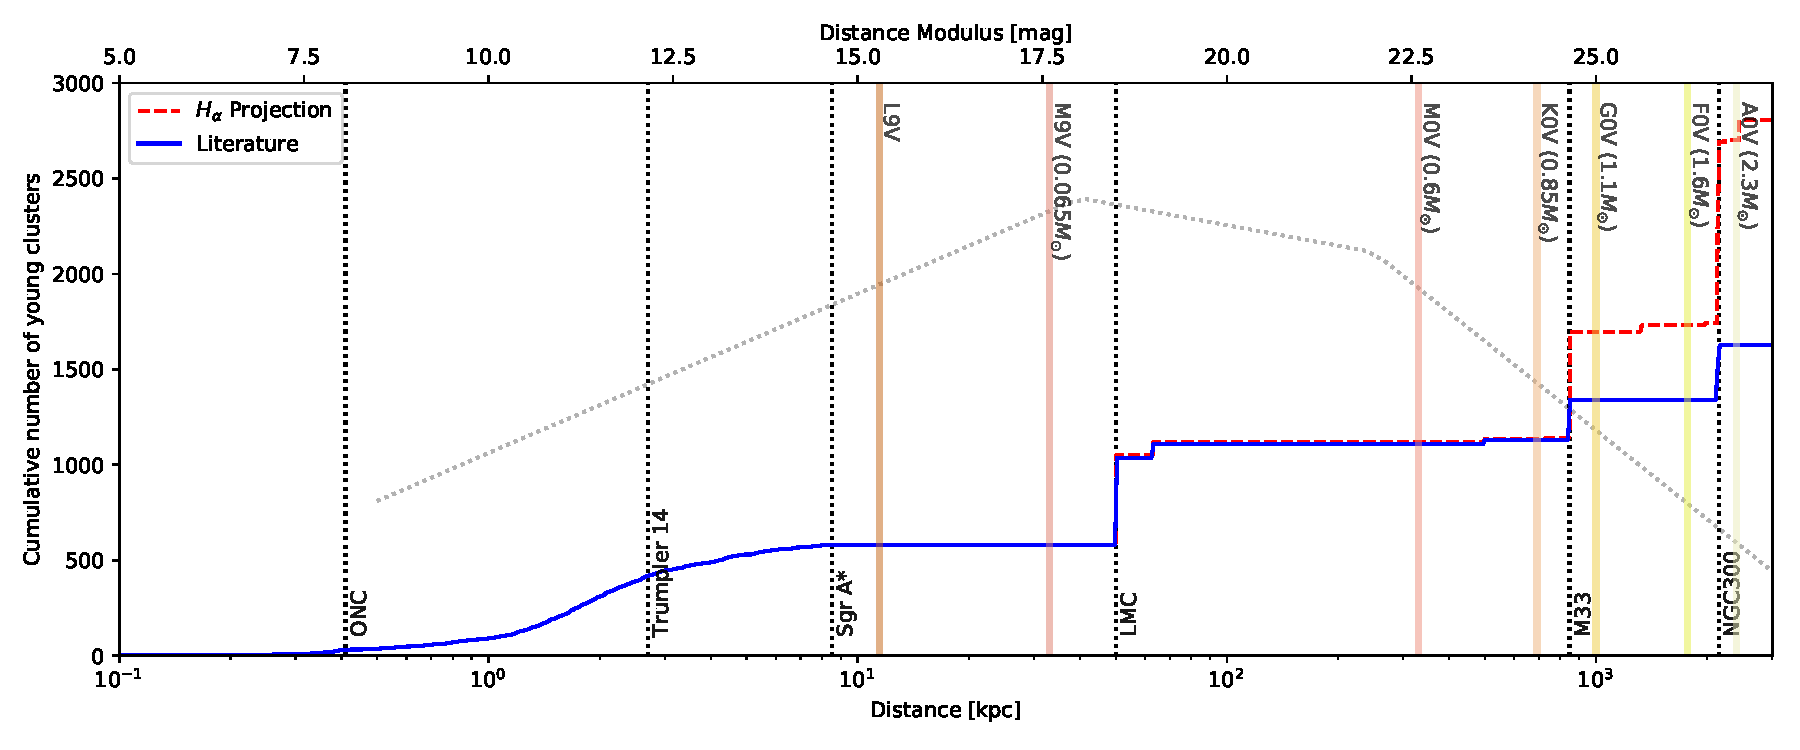
\includegraphics[width=\textwidth]{images/young_clusters_within_2Mpc_incl_MW.pdf}

    \caption{Cumulative number of young cluster targets that will be available to MICADO (\textdelta\,\textless\,+35\textdegree) out to 2 Mpc. The blue line show the cumulative number of young clusters with increasing distance from Earth as reported in catalogues and the literature (see references in Table \ref{tbl:cum_cluster_refs}.
    The red dotted line shows the expected number of young clusters in a given galaxy based on an extrapolation of a galaxy's star formation rate from its total H$_\alpha$ flux \citep{caldwell09}.
    The solid vertical lines represent the observational horizons for given stellar spectral types assuming a detection limit of K=28$^m$ with MICADO at the ELT. The faint dotted grey line shows the corresponding approximation distance limits for determining the slope of various regions of the IMF using MICADO.
    The population of Milky Way clusters is taken from the HEASARC Milky Way Open Cluster database \citep{heasarc_mwsc} and represents only the clusters located at declinations accessible to MICADO (-85\textdegree\,\textless\,\textdelta\,\textless\,+35\textdegree)
    }
    \label{fig:local_group_cluster_number}

\end{figure*}

\citet{portegies2010} provides a curated list of the most well known massive young clusters in- and outside the Milky Way. However many more clusters exist within the local group of galaxies. 
Indeed to fully understand the environmental dependence on cluster formation and evolution, a statistically large number of extra-galactic clusters will need to be observed. 
Figure \ref{fig:local_group_cluster_number} shows the pool of clusters available to MICADO at the ELT along with the corresponding observational limits of stars of various masses. 
Within the Mily Way alone, over 500 star clusters become available for which a fully resolved IMF (including the Brown Dwarf regime) could be determined. 
If the Magellanic clouds are included for studying the region either side of the IMF peak, this number increases to over 1000 young cluster targets. 
Out to 2Mpc the resolved high-mass slope of the IMF could be studied in between 1500 and 2500 clusters, including up to 1000 new previously undocumented star clusters\footnote{This estimate is based on each galaxy's total H$_\alpha$ flux with the conversion to approximate number of clusters based on the H$_\alpha$ derived star formation rate and young cluster catalogue for M31 \citep{caldwell09}.}.

MICADO will enable IMF studies of fully resolved populations to move from direct IMF measurements of single clusters in and around the solar neighbourhood to statistically large numbers of clusters in a diverse set of environments both in- and outside the Milky Way. Such a statistically meaningful sample of resolved IMFs will hopefully enable a robust determination of any environmental parameters that influence the star formation process, thus answering the major open question of IMF universality.

% The blue curve in Figure \ref{fig:local_group_cluster_number} shows the cumulative number of possible MICADO targets reported in catalogues and the literature for both the Milky Way and in galaxies out to 2 Mpc (for references see Table A\ref{tbl:cum_cluster_refs}). 
% The red dotted curve adds the approximate number of additional clusters in the local group which have not yet been catalogued. 
% 
% What is evident from Figure \ref{fig:local_group_cluster_number} is that there
% exist hundreds (potentially thousands) of clusters within a 2 Mpc radius that will
% be observable by MICADO, which could be used for a statistical analysis of the IMF
% under varying environmental conditions. 



% Milky way cluster numbers are taken from the HEASARC MWOCDB
% Extra-galactic cluster numbers are taken from the references in table 

% Makes a plot of cumulative star formation vs distance. This SFR is converted
% into an "average number of clusters", assuming the 140 M31 number of SF regions
% can be equivalent to a SFR of 0.5 Msun / yr.
% See Caldwell 2009 \citep{caldwell09}, 140 young clusters in M31 @ 0.5 Msun/yr

% The number of galaxies that will be seen by MICADO are limited by the latitude
% of Armazones: -25 deg +/- 60 deg --> [-85, +35]


% \begin{figure*}

%     \centering
%     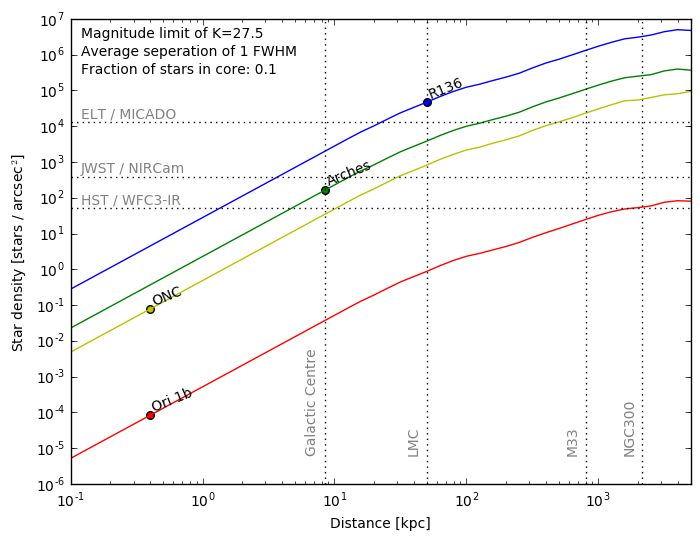
\includegraphics[width=\textwidth]{images/star_density_motivation}

%     \caption{}
    
%     \label{fig:resolved_stellar_densities}
    
% \end{figure*}


% What is the lowest mass star that MICADO will be able to observe for a given density and distance? 
% How crowded can a region be for MICADO to still be able to detect 90% of the stars above the detection limit? 
% What instrumental effects will play a critical role when undertaking such studies with MICADO and the ELT?


% Results}
% - 
% * ELT PSFs make life very difficult - many fake sources
% * MICADO can get well into the Brown dwarf regime (>0.01Msun) for all clusters within 8kpc of the Sun
% * It will just miss out on the BD knee in the LMC (>0.1Msun). But it will catch the true structure of the 0.5Msun knee.
% * Densities of ~1000 stars/arcsec2 are easily resolvable. 5000 stars/arcsec2 if we have good knowledge of the PSF.
% * This is equivalent to every star in the Arches cluster at a distance of the LMC. ONC would be fully resolvable (assuming no extinction) in Leo I Dwarf (220kpc)
% * in the LMC, meaning MICADO can basically resolve out all stars in every YMC listen in Portegeis-Zwart 2010



% NEED COMPLETENESS NUMBERS - HOW MANY ACTUALLY CAME BACK!!!!

    % - At what densities does the PSF subraction break down?

    % - At what desntites do we start getting fake sources from the PSF artifacts?

% - What is the limiting mass vs distance vs stellar density

% - What are the effective densities for the cases where the limiting mass is resolution limited?
% - Where does JWST drop out?

    % - Examples of the clusters (i.e. ONC in NGC300) where MICADO will make the biggest contribution
    
% - What level of variation in each mass regime (M<0.08, 0.08<M<0.5, M>0.5) do we see?

%\section{Discussion}
\label{sec:discussion}




- To which distance can go below the Hydrogen-burning limit?

- To which distance can go go below the 0.5 Msun knee?

- How far down can we go in Local group spiral galaxies? e.g. NGC300?

- Is it possible to claim variation is the data?


- What are the dangers of not having a proper PSF?

- What are the dangers of binning?

- How to avoid extracting fake sources? Rotational dithering?
\section{Conclusion}
\label{sec:conclusion}

MICADO and the ELT will provide the chance to finally resolve the core populations of the densest star clusters in the Milky Way and neighboring galaxies out to distances of several hundred kiloparsecs \textcolor{red}{isn't it 5 Mpc?}.  With MICADO observations of young stellar clusters, one can finally answer the question as to whether the IMF distribution is indeed universal, or whether its shape changes when we leave the solar neighborhood. Currently, these answers are locked inside the dense cores of young stellar clusters, as observations of these clusters are primarily limited by confusion.

The main goal of this work was to determine precisely how much more of these stellar populations will be visible to MICADO. We tried to answer three questions: What is the lowest mass star that MICADO will be able to observe reliably for a given stellar density and distance? What instrumental effects will play a critical role? How many clusters will be available for IMF studies? In order to answer these, we used the instrument simulator for MICADO (SimCADO) to generate synthetic observations of 56 dense stellar regions corresponding to the cores of young stellar clusters at varying distances from Earth. Here we present a summary of the results:

\begin{enumerate}
    \item We have shown that MICADO will easily be able to resolve all members of a stellar population with a density up to 10\h3\,\spa. With proper knowledge of the PSF and an optimized detection and subtraction algorithm densities of 5$\times$10\h3\,\spa should also be achievable.
    
    \item Observations with MICADO will enable direct (resolved) observations of the IMF in well over 1500 young clusters in diverse environments within the local group of galaxies. These observations will provide a statistically meaningful sample for robustly quantifying possible IMF variations and the role of environment on the shape of the IMF.

    % \item Given that MICADO observations will be constrained by the sensitivity to both the brightest and faintest sources in the field of view, MICADO is best suited to investigate the shape of the IMF in clusters in the outer edges of the Milky Way as well as the Magellanic Clouds. For example, MICADO is ideally suited to resolve the IMF in cores of dense young star clusters such as R136 in the LMC and NGC330 in the SMC.
    
    \item MICADO's resolution will allow the peak of the IMF (0.1\,\msun\textless M \textless0.5\,\msune) to be extensively investigated in the Magellanic clouds, and the Salpeter slope of the high mass region of IMF out to distances of 5\,Mpc (M83).
    
    \item Observations focusing on the initial mass function of clusters in the LMC will be limited by sensitivity, not crowding, to 0.1\,\msun. 
    
    \item Investigations of the transition around the hydrogen burning limit (\s0.08\,\msun) will not be possible outside the Milky Way. Instead, brown dwarf populations will be accessible in the cores of the densest Milky Way clusters, e.g. in the Westerlund clusters or the emerging W49A clusters. Objects with masses on the order of 10\,M$_{Jup}$ will be accessible by MICADO for clusters within 8\,kpc of Earth. The only caveat is that an appropriate observation strategy must be found to mask the many bright (m$_{Ks}<15^m$) stars present in all Milky Way clusters.    
    
    \item Finally, accurate knowledge of the ELT's PSF will be absolutely essential for good photometry and PSF subtraction algorithms. The sharp structures created by the segmented mirror design will lead to many fake low luminosity star detections if either the PSF is not well known or the extraction algorithm is not capable of differentiating between a star and an artifact of the PSF.
    
\end{enumerate}


% The parameter space covered distances from 8\,kpc to 5\,Mpc and stellar densities from 10\h2\,\spa to \s10\h5\,\spa - densities much higher then either Hubble or JWST will be capable of resolving. 


% - Answer the questions in the introduction

    % - At distance X and for stellar density Y, down to which mass (Z) can I get an IMF?
    
    % - If variations exist in the IMF, what level could MICADO detect at which distance?
    
% - Brief comparison to JWST's capabilities and where MICADO will accel

% - Brief note on how important the need for PSF-Reconstruction is and how we need to develop tools for source detection and extraction which can properly deal with non-smooth PSFs

\begin{acknowledgements}

KL would also like to express his gratitude to Gijs Verdoes Kleijn, Eline Tolstoy, and Ric Davies for the insightful and helpful comments and discussions regarding future possible observations with the ELT.

SimCADO incorporates Bernhard Rauscher's HxRG Noise Generator package for python \citep{nghxrg}. 
This research made use of POPPY, an open-source optical propagation Python package originally developed for the James Webb Space Telescope project \citep{poppy}. 
This research made use of Astropy, a community-developed core Python package for astronomy \citep{astropy, astropy2}. 
This research made use of Photutils \citep{photutils}. 
This research has made use of ``Aladin sky atlas'' developed at CDS, Strasbourg Observatory, France \citep{aladin, aladinlite}.
SimCADO makes use of atmospheric transmission and emission curves generated by ESO's SkyCalc service, which was developed at the University of Innsbruck as part of an Austrian in-kind contribution to ESO. 

This research is partially funded by the project IS538003 of the Hochschulraumstrukturmittel (HRSM) provided by the Austrian Government and administered by the University of Vienna.

\end{acknowledgements}
\bibliographystyle{aa}
\bibliography{imf_refs}

% \appendix
\begin{appendix}

%%%%%%%%%%%%%%%%%%%%%%%%%%%%%%%%%%%%%%%%%%%%%%%%%%%%%%%%%%55
% Core size and density from Portegeis-Zwart 2010
\section{Supplemental material}

\begin{table*}
    \centering
    \caption{The age and observable stellar densities for a selection of young massive clusters found both in and outside the Milky Way, as listed in \citet{portegies2010}. The densities have been calculated to only include stars which are brighter than Ks=28\m, as fainter stars will not be detectable by MICADO. The table list the parameters for the clusters shown in Fig. \ref{fig:star_density_vs_age}.}
    \label{tbl:pz10_selection}
    \begin{tabular}{l l r r r r r r}
        \hline\hline
        Galaxy & Cluster      & Distance & Age  & log(Mass) & Core radius & log$_{10}$($\rho$)    & Limiting mass \\
               &              & kpc      & Myr  & \msun     & arcsec  & stars arcsec\h{-2} & \msun         \\
        \hline
        \multicolumn{8}{c}{Cores resolvable by HST}                                                     \\
        \hline
        MW     & ONC          & 0.4      & 1    & 3.7       & 100     & -1.6           & 0.01          \\
        \hline
        \multicolumn{8}{c}{Cores resolvable by JWST}                                                    \\
        \hline
        MW     & Trumpler-14  & 2.7      & 2    & 4         & 10.7    & 1.1            & 0.01          \\
        MW     & Quintuplet   & 8.5      & 4    & 4.0       & 24      & 1.1            & 0.04          \\
        MW     & NGC3603      & 3.6      & 2    & 4.1       & 8.6     & 1.2            & 0.01          \\
        MW     & Westerlund-1 & 5.2      & 3.5  & 4.5       & 15.9    & 1.7            & 0.01          \\
        LMC    & NGC2214      & 50       & 39.8 & 4.0       & 7.5     & 1.9            & 0.1           \\
        \hline
        \multicolumn{8}{c}{Cores resolvable by MICADO}                                                  \\
        \hline
        LMC    & NGC1847      & 50       & 26.3 & 4.4       & 7.1     & 2.2            & 0.1           \\
        LMC    & NGC2157      & 50       & 39.8 & 4.3       & 8.2     & 2.2            & 0.1           \\
        LMC    & NGC1711      & 50       & 50.1 & 4.2       & 7.9     & 2.2            & 0.1           \\
        LMC    & NGC1818      & 50       & 25.1 & 4.4       & 8.5     & 2.3            & 0.1           \\
        LMC    & NGC2164      & 50       & 50.1 & 4.2       & 6.1     & 2.3            & 0.1           \\
        SMC    & NGC330       & 63       & 25.1 & 4.6       & 7.7     & 2.4            & 0.15          \\
        LMC    & NGC2136      & 50       & 100  & 4.3       & 6.6     & 2.4            & 0.1           \\
        MW     & Arches       & 8.5      & 2    & 4.3       & 4.9     & 2.5            & 0.04          \\
        LMC    & NGC1850      & 50       & 31.6 & 4.9       & 11      & 2.5            & 0.1           \\
        LMC    & NGC2004      & 50       & 20   & 4.4       & 5.8     & 2.5            & 0.1           \\
        LMC    & NGC2100      & 50       & 15.8 & 4.4       & 4.1     & 2.7            & 0.1           \\
        M31    & B257D        & 780      & 79.4 & 4.5       & 0.8     & 3.4            & 0.9           \\
        \hline
        \multicolumn{8}{c}{Only outer regions resolvable by MICADO}                                    \\
        \hline
        LMC    & R136         & 50       & 3    & 4.8       & 0.41    & 3.7            & 0.1           \\
        M31    & B066         & 780      & 70.8 & 4.3       & 0.10    & 4.2            & 0.9           \\
        M31    & B040         & 780      & 79.4 & 4.5       & 0.15    & 4.3            & 0.9           \\
        M31    & B043         & 780      & 79.4 & 4.4       & 0.19    & 4.3            & 0.9           \\
        M31    & B318         & 780      & 70.8 & 4.4       & 0.05    & 4.4            & 0.9           \\
        M31    & B448         & 780      & 79.4 & 4.4       & 0.05    & 4.4            & 0.9           \\
        M31    & Vdb0         & 780      & 25.1 & 4.9       & 0.37    & 4.4            & 0.9           \\
        M31    & B327         & 780      & 50.1 & 4.4       & 0.05    & 4.5            & 0.9           \\
        M31    & B015D        & 780      & 70.8 & 4.8       & 0.06    & 4.6            & 0.9           \\
        \hline
    \end{tabular}
\end{table*}


%%%%%%%%%%%%%%%%%%%%%%%%%%%%%%%%%%%%%%%%%%%%%%%%%%%%%%%%%%%%%%%%%%%%%%%%%%%%%%%%
% References for the cumulative cluster numbers within 2 Mpc

\begin{table*}
    \centering
    \caption{References for the cumulative cluster numbers within a 2 Mpc radius
    which will be observable by MICADO at the ELT. Star formation rate estimates 
    are based on the integrated galaxy $H_{\alpha}$ fluxes from \citet{karachentsev2013}
    and were used to estimate the true number of open clusters contained in each
    galaxy. The Milky Way clusters were taken from the HEASARC Milky Way Star Cluster
    catalogue \citep{heasarc_mwsc} and filtered to only include clusters visible to 
    MICADO at the ELT (i.e. Dec $<$ +35 deg).
    }
    \label{tbl:cum_cluster_refs}
    \begin{tabular}{lrrrl}
    
    \hline
    \hline
    Name     & SFR                  & Distance  & N Clusters & Reference      \\
             & [M$_\odot$ / yr]     & [kpc]     &            &                \\
    \hline
    MilkyWay &                      & 8         & 590        & Kharchenko+13  \\
    LMC      & 0.30                 & 50        & 456        & Glatt+10       \\
    SMC      & 0.05                 & 63        & 71         & Glatt+10       \\
    NGC6822  & 0.01                 & 499       & 24         & Karampelas+09  \\
    M33      & 0.36                 & 847       & 208        & Fan+14         \\
    NGC0055  & 0.45                 & 2128      & 168        & Castro+08      \\
    NGC0300  & 0.18                 & 2148      & 117        & Pietrzynski+01 \\
    NGC4214  & 0.15                 & 2938      & 52         & Andrews+13     \\
    \hline
    \end{tabular}
\end{table*}





%Figures A\ref{fig:results_lmc_1E3} and A\ref{fig:results_lmc_1E4} show the results for two of the 42 simulated observations. Both figures show the case of a cluster located at the distance of the LMC. In each figure the observation of the cluster can be seen along side the residuals of the subtraction process. For clusters with densities lower than 10\h3 stars arcsec\h{-2} the subtraction process worked very well, with almost all stars being accurately removed (see Fig A\ref{fig:results_lmc_1E3}). After this level the effectiveness of the PSF subtraction continually degraded with increasing density. This was to be expected. Figure A\ref{fig:results_lmc_1E4} shows the case for a 10\h4 stars arcsec\h{-2} cluster. Although the majority of stars were removed from the image, the stars which failed the fitting test remain. This was often due to two sufficiently bright stars being too close together and the fitting algorithm was not able to match a symmetrical Gaussian profile to the pair. These failed subtractions had a knock-on effect where the fainter artefacts of the PSF were detected as stars with lower signal to noise ratios, which increased the number of fake source detections. The bottom right panels Figures A\ref{fig:results_lmc_1E3} and A\ref{fig:results_lmc_1E4} shows the ratio of real mass to detected mass for each of the stars extracted from the simulated images, as well as the standard deviation for the mass ratio bins. It can be seen that the standard deviation is a good indicator for extraction reliability.


\begin{figure*}
    \centering
    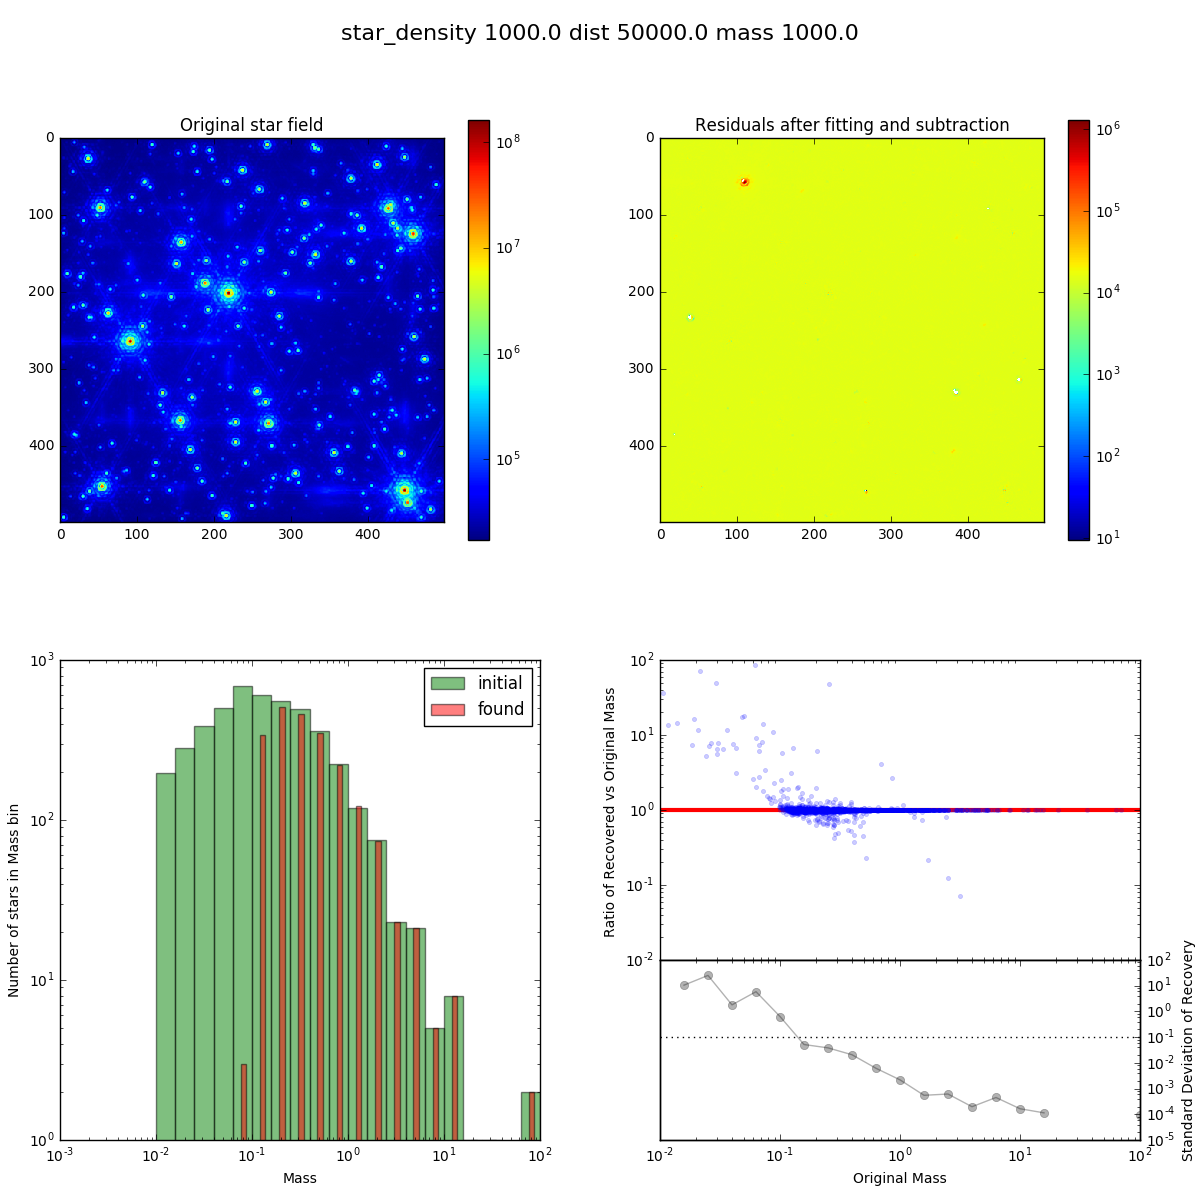
\includegraphics[width=\textwidth]{images/results6_dist=50000_rho=1000}
    \caption{Results of extracting stars from a 1000\,\spa cluster at a distance of 50\,kpc. Top left: The original 2''$\times$2'' stellar field with a density of 10\h3~\spa. The stars in the field have masses between 0.01\,\msun and 300\,\msune. The PSF used in this study was an instantaneous SCAO PSF, similar to what would be seen on a single MICADO detector 2.6\,s exposure. Top right: The same field after our detection and subtraction algorithm has iteratively removed all the stars. 10\h3~\spa are extracted reasonably easily by our algorithm. Bottom left: The fraction of extracted stars in each mass bin which matched up with the original list of stars. The majority of stars more massive than 0.1\,\msun were detected. Bottom right: The upper panel shows the ratio of extracted mass to original mass. The vast majority (\s97\%) of the almost 4000 stars in the image fell almost perfectly on the red one-to-one line. The minor scatter around the line is due to a combination of our detection algorithm not being able to discern between to very close stars, and contamination for the PSF artefacts, e.g. the segmented diffraction spikes. The lower panel shows the standard deviation of masses around the one-to-one line in a certain mass bin. A mass bin was deemed reliable if the average recovered to original mass ratio was in the range 1$\pm$0.1 and the standard deviation was less than 10\%.}
    \label{fig:results_lmc_1E3}
\end{figure*}


\begin{figure*}

    \centering
    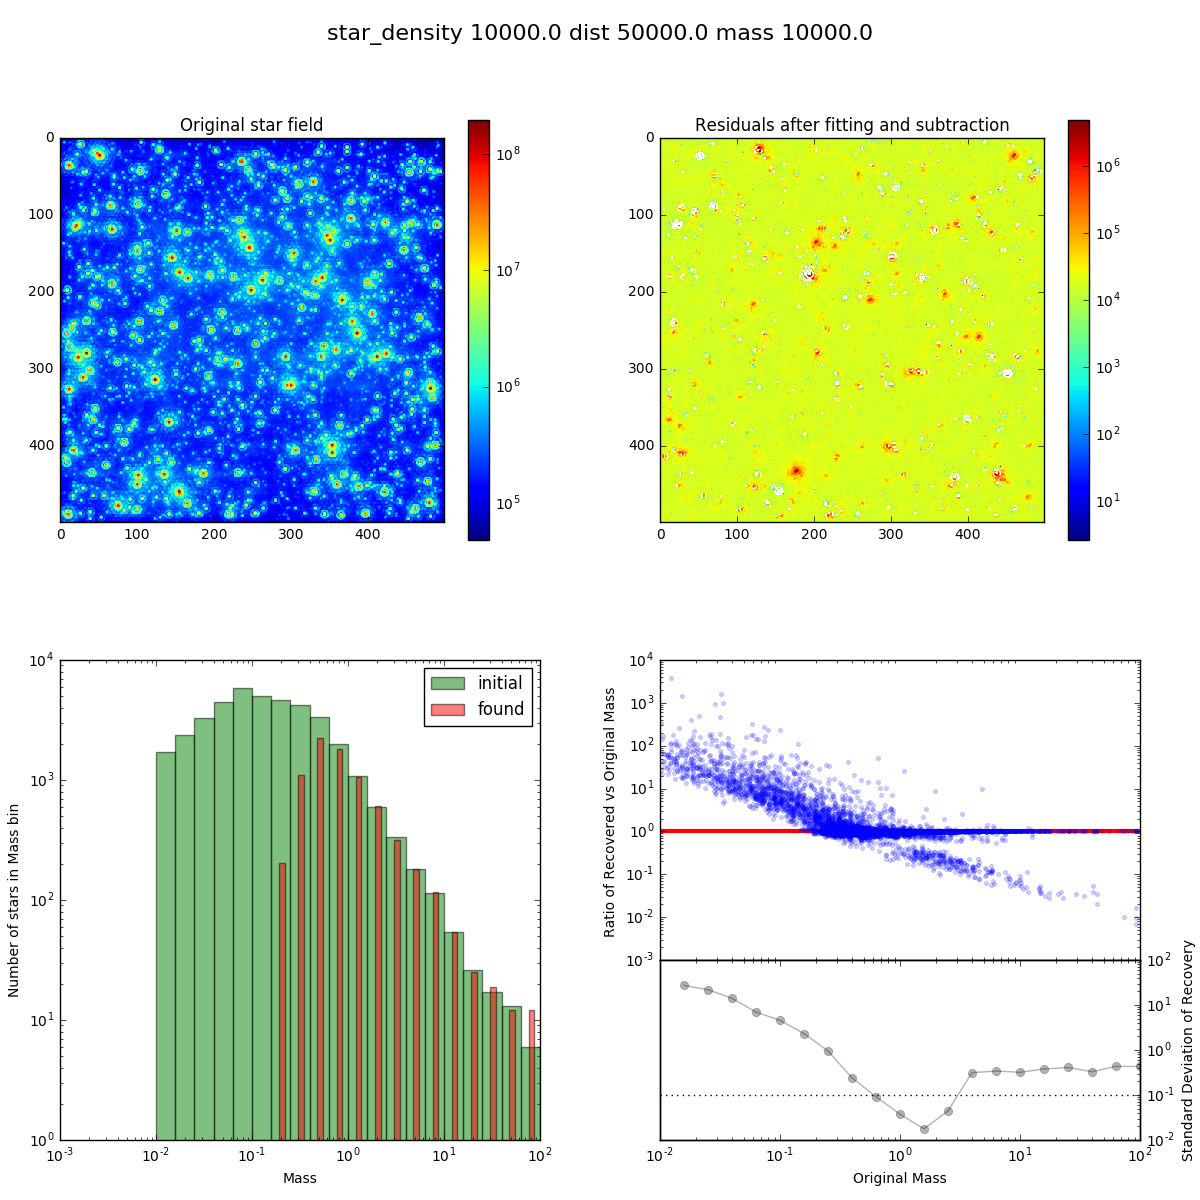
\includegraphics[width=\textwidth]{images/results6_dist=50000_rho=10000}

    \caption{Same as Fig. \ref{fig:results_lmc_1E3} but for a stellar density of 10\h4~\spa. At these densities the number of ``double'' stars has increased to the point where our detection algorithm was unable to accurately fit and subtract many of the bright stars. Although a large number of incorrect mass determinations are visible in the big blue cloud, still around 60\% of the \s40\,000 sources in this image fall on the red one-to-one line. The segmented PSF meant that the the algorithm detected many fake sources which skewed the detection statistics in both the high and low mass regimes. We are still looking into ways of preventing this from happening in future studies.}
    
    \label{fig:results_lmc_1E4}
    
\end{figure*}

\end{appendix}



%________________________________________________________________

\end{document}